\documentclass[11pt]{article}

\usepackage{amsmath}
\usepackage{amsfonts}
\usepackage{amssymb}
\usepackage{graphicx}
\usepackage{hyperref}
\usepackage[margin=2cm]{geometry}
\usepackage{multirow}



\title{Strong coupling between scales in a multi-scalar model of urban dynamics}


\author{Juste Raimbault$^{1,2,3,\ast}$\medskip\\
$^{1}$ Center for Advanced Spatial Analysis, University College London\\
$^{2}$ UPS CNRS 3611 ISC-PIF\\
$^{3}$ UMR CNRS 8504 G{\'e}ographie-cit{\'e}s\medskip\\
$^{\ast}$ \texttt{juste.raimbault@polytechnique.edu}
}

\date{}


\begin{document}


\maketitle


\begin{abstract}
	Urban evolution processes occur at different scales, with intricate interactions between levels and relatively distinct type of processes. To what extent actual urban dynamics include an actual strong coupling between scales, in the sense of both top-down and bottom-up feedbacks, remains an open issue with important practical implications for the sustainable management of territories. We introduce in this paper a multi-scalar simulation model of urban growth, coupling a system of cities interaction model at the macroscopic scale with morphogenesis models for the evolution of urban form at the scale of metropolitan areas. Strong coupling between scales is achieved through an update of model parameters at each scale depending on trajectories at the other scale. The model is applied and explored on synthetic systems of cities. Simulation results show a non-trivial effect of the strong coupling. As a consequence, an optimal action on policy parameters such as containing urban sprawl is shifted. We also run a multi-objective optimization algorithm on the model, showing showing that compromise between scales are captured. Our approach opens new research directions towards more operational urban dynamics models including a strong feedback between scales.
	\medskip\\
\textbf{Keywords: } Urban dynamics; Systems of cities; Urban morphogenesis; Multi-scalar modeling; Strong coupling
\end{abstract}

%  relevant target CEUS? https://www.elsevier.com/journals/computers-environment-and-urban-systems/0198-9715/guide-for-authors => special issue expired; IJGI 31/01:  https://www.mdpi.com/journal/ijgi/special_issues/spatio_temporal_models_geo

% Systems of cities
%Multi-scalar model
%Spatial interaction
%Reaction-diffusion

% abstract CCS
% 
%The modeling of urban growth is a crucial issue for the design of sustainable territorial policies, through the understanding of past urbanization processes and the forecasting of future urban trajectories. Several models have been proposed at different scales and integrating differ- ent dimensions of urban systems, such as land-use transport interaction models [1] or systems of cities models [2]. While multi-scalar models are recognized as crucial for the study of such systems [3], they remain in practice unexplored.
%This contribution introduces a parsimonious multi-scalar model for systems of cities, based on simple dimensions (mainly populations) with stylized processes, but yielding an effective strong coupling between the metropolitan mesoscopic scale and the macroscopic scale of the system of cities. The model couples the spatial interaction model of [4] for the macro scale with the reaction-diffusion model for urban form studied by [5]. More precisely, urban areas viewed as a population grid are embedded into the macroscopic interaction model. To evolve populations and local urban forms, one time step consists of (i) population differences are computed by the interaction model; (ii) top-down feedback modifies parameters of mesoscopic models, given control parameters to capture typical scenarios (transit-oriented development or sprawl for diffusion, metropolization or uniformization for aggregation); (iii) local urban form are evolved with the reaction-diffusion models at a given speed conditionally to the population variations; (iv) changes in urban form influence macroscopic interaction ranges (capturing the impact of local activity on global insertion), by integrating gravity flows in the area with a squared cost function making a compromise between congestion and flows.
%The model is applied on synthetic systems of cities typical of a continental range (500km, hierarchy around 1, 20 cities), with initial local population grid configurations as monocen- tric. Parameter space is explored with the OpenMOLE model exploration software [6], eased by the implementation of the model in scala [7]. First results show a strong impact of the strong meso-macro coupling, such as for example a qualitative inversion of the behavior as a function of interaction range of macroscopic indicators trajectories when switching from a “transit-oriented development” scenario (negative feedback of population growth on diffusion) to a “sprawl” scenario (positive feedback). Similarly, mesoscopic urban form indicators are significantly influenced by the coupling process.
%Further work will consist in more targeted simulation experiments, including specific ex- ploration algorithms such as diversity search for model regimes [6], to test the model as a proof-of-concept of models for policies. Such a model can also be calibrated on real city sys- tems and urban form trajectories, to extrapolate coupling parameters that would be difficult to obtain otherwise. Our contribution is thus a first step towards multi-scalar simulation models for systems of cities.



% multilevel models : check https://scholar.google.fr/citations?user=x1BwVXoAAAAJ&hl=fr
% + Morvan, G. (2014). Bibliographic database on multi-level and multi-scale agent-based modeling. Transportation Research Procedia, 2, 495-500.

%\cite{louail2010comparer}

\section{Introduction}

The modeling of urban growth and more generally the dynamics of urban systems is central to the design of sustainable territorial policies, through the understanding of past urbanisation processes and the anticipation of future urban trajectories. The design of sustainable future cities requires an historical knowledge of how past cities came to be and evolved \cite{batty2018inventing}. Several models have been proposed at different scales and integrating different dimensions of urban systems, such as models of land-use change at a mesoscopic scale or systems of cities models at a macroscopic scale \cite{pumain2017urban}.

At the scale of a metropolitan area, Land-use Transport Interaction models \cite{wegener2004land} are for example a widely used tool to estimate the dynamics of spatial distributions of activities (mostly residential location and economic activities) in response to an evolution of the accessibility landscape caused by new transportation infrastructures \cite{raimbault:halshs-02265423}. In a similar context, cellular automata models of urban growth or land-use change study more generally land-use transitions with a high spatial resolution, and are mostly data-driven \cite{clarke2007decade}. At the smaller scale of the system of cities, macroscopic models of urban growth have focused on reproducing the distribution of city sizes, either through economic processes as e.g. \cite{gabaix1999zipf}, or from a geographical point of view focusing on interactions between cities \cite{favaro2011gibrat}.

Territorial dynamics, and more particularly urban dynamics, have according to \cite{pumain1997pour} an intrinsic multi-scalar nature, with successive autonomous levels of emergence from individual microscopic agents to the mesoscopic scale of the city and the macroscopic scale of the system of cities. While models at each scale with distinct ontologies are useful to answer their own questions, an explicit account of inter-scale feedbacks, both top-down and bottom-up, would allow testing policies and interventions distributed and differentiated across scales while not neglecting the interactions between scales \cite{wegener2018multi}. Indeed, the need for sustainable territorial policies would imply the construction of multi-scalar models to take simultaneously into account issues associated to each relevant scale \cite{Rozenblat2018,raimbault:halshs-02284933}.


% rq: no def nor clarification of what is meant by "scale"!

Multi-scalar models of urban dynamics are however still at their beginnings. \cite{murcio2015urban} consider population flows at different spatial ranges from the urban area to the country, but does not incorporate distinct ontologies and processes for the different scales. \cite{batty2005agents} however suggests that a similar formalism can be applied to urban processes at different scales. Multi-level statistical models capture some information at imbricated scales \cite{shu2020modelling}, although they can not be used as dynamical simulation models. Similarly, multi-level cellular automata (CA) models for urban growth include factors influencing urban expansion at multiple scales \cite{xu2019directional}. \cite{cheng2003modelling} propose a general framework for such approaches. \cite{torrens2001cellular} suggest that hybrid models coupling CA with other formalisms is a crucial development in the field. \cite{white2006modeling} introduces a CA with variable grid size to account for heterogeneities across scales. \cite{zhu2020dynamic} couple an agent-based model with a CA at multiple scales. \cite{yu2018modeling} embed a local CA into a regional intercity model and a macroscopic potential model. \cite{ford2019multi} couple at different scales an urban development model with a flooding risk model to forecast the future impact of extreme climate events on the London metropolitan region. \cite{xu2020urban} develop an agent-based model of urban expansion with both macro and micro agents. \cite{raimbault:halshs-02013006} suggests that integrating network dynamics at the link level in a macroscopic urban system models is a way to implement a multi-scale model, as done by \cite{raimbault2020hierarchy} which explores hierarchy properties of cities and networks in this context.

In disciplines neighbour to urban modeling, methods have been developed for multi-scale models. For example in spatial epidemiology, \cite{banos2015importance} combines agent-based modeling for local diffusion dynamics with differential equations at the population scale. The NetLogo software for agent-based modeling includes a specific extension for multi-scale modeling \cite{hjorth2020levelspace}. Multi-scale models have also been used for the simulation of crowd dynamics \cite{crociani2016multi}. The study of traffic is also made more accurate by coupling macroscopic and microscopic models \cite{boulet2020coupling}. The management of ecosystems  requires integrating across actors and scales \cite{belem2013organizational}. These non-exhaustive illustrations highlight how the integration of scales is a crucial feature and issue in the understanding of complex systems \cite{chavalarias2009french}.


This paper contributes to the open question of multi-scalar models of urban dynamics by introducing a new simulation model which integrates a strong coupling between the mesoscopic scale and the macroscopic scale. The dynamics within each scale influence the other and reciprocally in an iterative way. More precisely, the model is simple in its components as we focus on the spatial structure of processes rather than on their multi-dimensionality. Therefore, we take into account only population variables, but both at the macroscopic scale of the system of cities and at the mesoscopic scale of the metropolitan area with an urban morphogenesis model. Our contribution is novel regarding previous works in particular regarding the following points: (i) the stylised model explicitly couples distinct scales and ontologies in a strong manner, most models operating only a weak coupling between scales (i.e. no reciprocal and dynamical feedbacks); (ii) the behavior of the model is systematically studied on synthetic systems of cities using model exploration methods.
 
% rq positioning: not large model but simple whih can be understood (cf requiem for large scale models)
 
The rest of this paper is organised as follows: we first describe the model; we then develop its exploration on synthetic systems of cities, and optimization using a genetic algorithm; we finally discuss developments and implications of this work.

% We describe in the following stylized facts justifying the approach => this could (should?) be an important development/basis for the work?

%Strong coupling and multi-scalarity 
%   Distinct processes and objects within each different scale
%   Weak inter-scale coupling, such as progressive resolution for land-use model, does not considers emergence and autonomous scales
% An integrated model, or strongly coupled, would be \textit{a new model extending the two coupled models in the sense that it includes them in some parameter settings or limit conditions}
%Urban multi-scalar complexity must be captured by a strongly coupled model
%no strongly coupled multi-scalar model in the literature (few examples such as  \cite{murcio2015urban} but without distinct ontologies)
%need to however consider ``simple'' models to be able to understand their behavior and extract knowledge from them
%\textbf{Research objective: }
%\textit{Investigate a strong coupling of a simple urban system interaction network at the macroscopic scale with an urban morphogenesis model at the mesoscopic scale}



\section{Multi-scale urban dynamics model}

\subsection{Rationale}

% ! reformulate - this is the CCS abstract

This contribution introduces a parsimonious multi-scalar model for systems of cities, based on simple dimensions (mainly populations) with stylized processes, but yielding an effective strong coupling between the metropolitan mesoscopic scale and the macroscopic scale of the system of cities.
The model couples the spatial interaction model of \cite{raimbault2018indirect} for the macro scale with the reaction-diffusion model for urban form studied by \cite{raimbault2018calibration}. More precisely, urban areas viewed as a population grid are embedded into the macroscopic interaction model. To evolve populations and local urban forms, one time step consists of (i) population differences are computed by the interaction model; (ii) top-down feedback modifies parameters of mesoscopic models, given control parameters to capture typical scenarios (transit-oriented development or sprawl for diffusion, metropolization or uniformization for aggregation); (iii) local urban form are evolved with the reaction-diffusion models at a given speed conditionally to the population variations; (iv) changes in urban form influence macroscopic interaction ranges (capturing the impact of local activity on global insertion), by integrating gravity flows in the area with a squared cost function making a compromise between congestion and flows.


% TODO figure
% 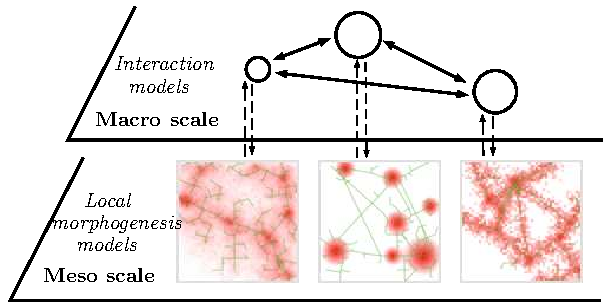
\includegraphics{figures/multiscale_morph.pdf}

\subsection{Formalization}


We consider $N$ urban areas, represented at the macroscopic scale by their population $P_j(t)$ at time $t$, and at the mesoscopic scale by a population grid $p_{kl}^{(j)}(t)$.

The model runs for a total number $t_f$ of time steps, and we will assume that $\Delta t = 1$ for the sake of simplicity (the formulas can be generalized for arbitrary values of the time step, for example when running on real data with irregular time sampling).

The system is initialized with synthetic data with a parameter $\alpha_0$ for the initial hierarchy, $P_0 (0)$ for the initial population of the largest city, in a square world of size $w$ (reference unit for the decay parameter).

At each time step:

\begin{enumerate}
	\item Aggregated population are evolved according to
	
	\begin{equation}
		P_i(t+1) = P_i(t) \left(1 + \Delta t \cdot \left(g_i + \frac{w_i}{N} \cdot \sum_j \frac{V_{ij}}{<V_{ij}>} \right) \right)
	\end{equation}
	
	where the gravity interaction potential is given by 
	
	\begin{equation}
		V_{ij} = \left(\frac{P_i P_j}{(\sum_k p_k)^2}\right)^{\gamma_G} \cdot \exp \left(- \frac{d_{ij}}{d_i} \right)
	\end{equation}

	and we write the population variations
	
	\begin{equation}
		\Delta P_i (t) = P_i (t + 1) - P_i (t)
	\end{equation}

	
	\item Mesoscopic parameters are modified following the evolution of population such that 
		\begin{itemize}
			\item the mesoscopic growth rate is adjusted to the population growth uniformaly over the time interval	
			    $N_G^{(i)} (t + 1) = \Delta P_i / t_m$
			\item The sprawl parameter evolves according to a fixed multiplier and the relative population increase following 
			\begin{equation}
				\beta_i (t+1) = \beta_i (t) \cdot \left(1 + \delta\beta \cdot \frac{\Delta P_i (t)}{\max_k  \Delta P_k (t)}\right)
			\end{equation}
			where the multiplier parameter $\delta\beta$ allows testing different scenarios: a negative value corresponds to transit-oriented development while a positive value corresponds to an uncontrolled sprawl
			\item The aggregation parameter evolves in a similar way but as a function of accessibility increase
			\begin{equation}
				\alpha_i (t+1) = \alpha_i (t) \cdot \left(1 + \delta\alpha \cdot \frac{\Delta Z_i (t)}{\max_k  \Delta Z_k (t)}\right)
			\end{equation}
			where the multiplier parameter $\delta\alpha$ allows switching between a metropolization scenario (more aggregation) and an uniformization scenario (less aggregation), and accessibility is given by
			\begin{equation}
				Z_i = \sum_j \frac{P_j}{\sum_k P_k} \cdot \exp( - d_{ij} / d_i)
			\end{equation}
			\item Change in the level of sprawl depends on the population pressure only, while aggregation depends on accessibility since it is linked to metropolization processes
			\item \textit{Note: the linear scale for these two parameters may not be relevant depending on the distribution of increments ?} $\rightarrow$ to be tested
		\end{itemize}
	
	\item Mesoscopic grids are evolved by the updated parameters, and $t_m$ time steps, following the aggregation-diffusion model, with $n_d$ unchanged. Slight differences in the end (due to rounding in computing the number of steps) is corrected by adjusting the macroscopic increments by the effective mesoscopic increments (which are assumed to be more precise).
	
	\item Macroscopic parameters are updated: for the sake of simplicity, only interaction decays are updated, assuming that urban form pattern play a role in the global insertion of the city. More precisely, we compute gravity flows within the area, and aggregate their value as an economic activity with a squared negative externality interpreted as a congestion with a cost $\lambda$ following
	
	\begin{equation}
		U_i = \sum_{kl} \left( \frac{P_k P_l}{P^2} \cdot \frac{1}{d_{kl}} - \lambda \left(\frac{P_k P_l}{P^2} \cdot \frac{1}{d_{kl}}\right)^2 \right)
	\end{equation}
	
	We do not add gravity parameter nor hierarchy parameter for the sake of simplicity. This utility $U_i$ is used to update the interaction decays following
	
	\begin{equation}
		d_i (t+1) = d_i (t) \left( 1 + \delta d \cdot \frac{U_i}{\max_k \left|U_k\right|} \right)
	\end{equation}
	where the multiplier parameter $\delta d$ allows controlling for the influence of local performance on global insertion.
\end{enumerate}





\subsection{Parameters}

The Table~\ref{tab:parameters} summarizes model parameters.

\begin{table}
	\caption{Summary of model parameters\label{tab:parameters}}
	\centering
	\begin{tabular}{|c|c|c|c|}
	\hline
		Type & Parameter & Process & Range \\\hline
		\multirow{4}{*}{Macro} & $g_i = g_0$ & Endogenous growth & \\
		& $w_i = w_G$ & Interactions weight & \\
		& $\gamma_i = \gamma_G$ & Interactions hierarchy & \\
		& $d_i$ & Interactions decay & \\ \hline
		\multirow{4}{*}{Meso} & $\alpha_i$ & Aggregation & \\
		& $\beta_i$ & Diffusion & \\
		& $t_m$ & Urban growth speed & \\
		& $n_d$ & Diffusion & \\ \hline
		\multirow{3}{*}{Multiscale} & $\delta\alpha$ & Downward feedback & \\
		& $\delta\beta$ & Downward feedback & \\
		& $\delta d$ & Upward feedback & \\\hline
	\end{tabular}
\end{table}


\subsection{Synthetic setup}

Model applied on synthetic systems of cities:


\begin{itemize}
	\item random positions and rank-size hierarchy ($\alpha \textrm{ = } 1.0$ and $P_0 \textrm{ = } 100,000$)
	\item countrywide urban system scale: 500km and 20 cities
	\item initial population grids as monocentric (grid of size 50 and center cell density 1000 units)
	\item simulated for 20 macroscopic time steps (order of magnitude of half a century)
\end{itemize}



\subsection{Indicators}

Model behavior is characterized using the following indicators:

\textit{Indicators at the macroscopic scale: distributions of population, accessibilities, centralities (summarized by average, hierarchy, entropy)}

\textit{Indicators at the mesoscopic scale: urban form captured by Moran index, average distance, hierarchy, entropy}



\section{Results}

\subsection{Implementation}

The model is applied on synthetic systems of cities typical of a continental range (500km, hierarchy around 1, 20 cities), with initial local population grid configurations as monocentric. Parameter space is explored with the OpenMOLE model exploration software \cite{reuillon2013openmole}, eased by the implementation of the model in scala \cite{model}.


\textit{Performance constraints: simulate $N$ mesoscopic morphogenesis models in parallel (macroscopic interactions are efficient as based on matrices)}

 model implemented in \texttt{scala} and integrated within a broader library (including implementations of \cite{raimbault2018indirect} \cite{raimbault2018calibration}

\cite{favaro2011gibrat} \cite{cottineau2015modular})

\textit{Large number of parameters and output indicators}


Model: \texttt{https://github.com/JusteRaimbault/UrbanGrowth-model}
  Project: \texttt{https://github.com/JusteRaimbault/UrbanGrowth}
  Simulation data: \texttt{https://doi.org/10.7910/DVN/IRHMQK}




\subsection{Statistical consistency}

% one factor sampling

%(min around 1 for 3 indicators, above 5 for 2 and around 0.5 for 2)}

\medskip

\begin{center}
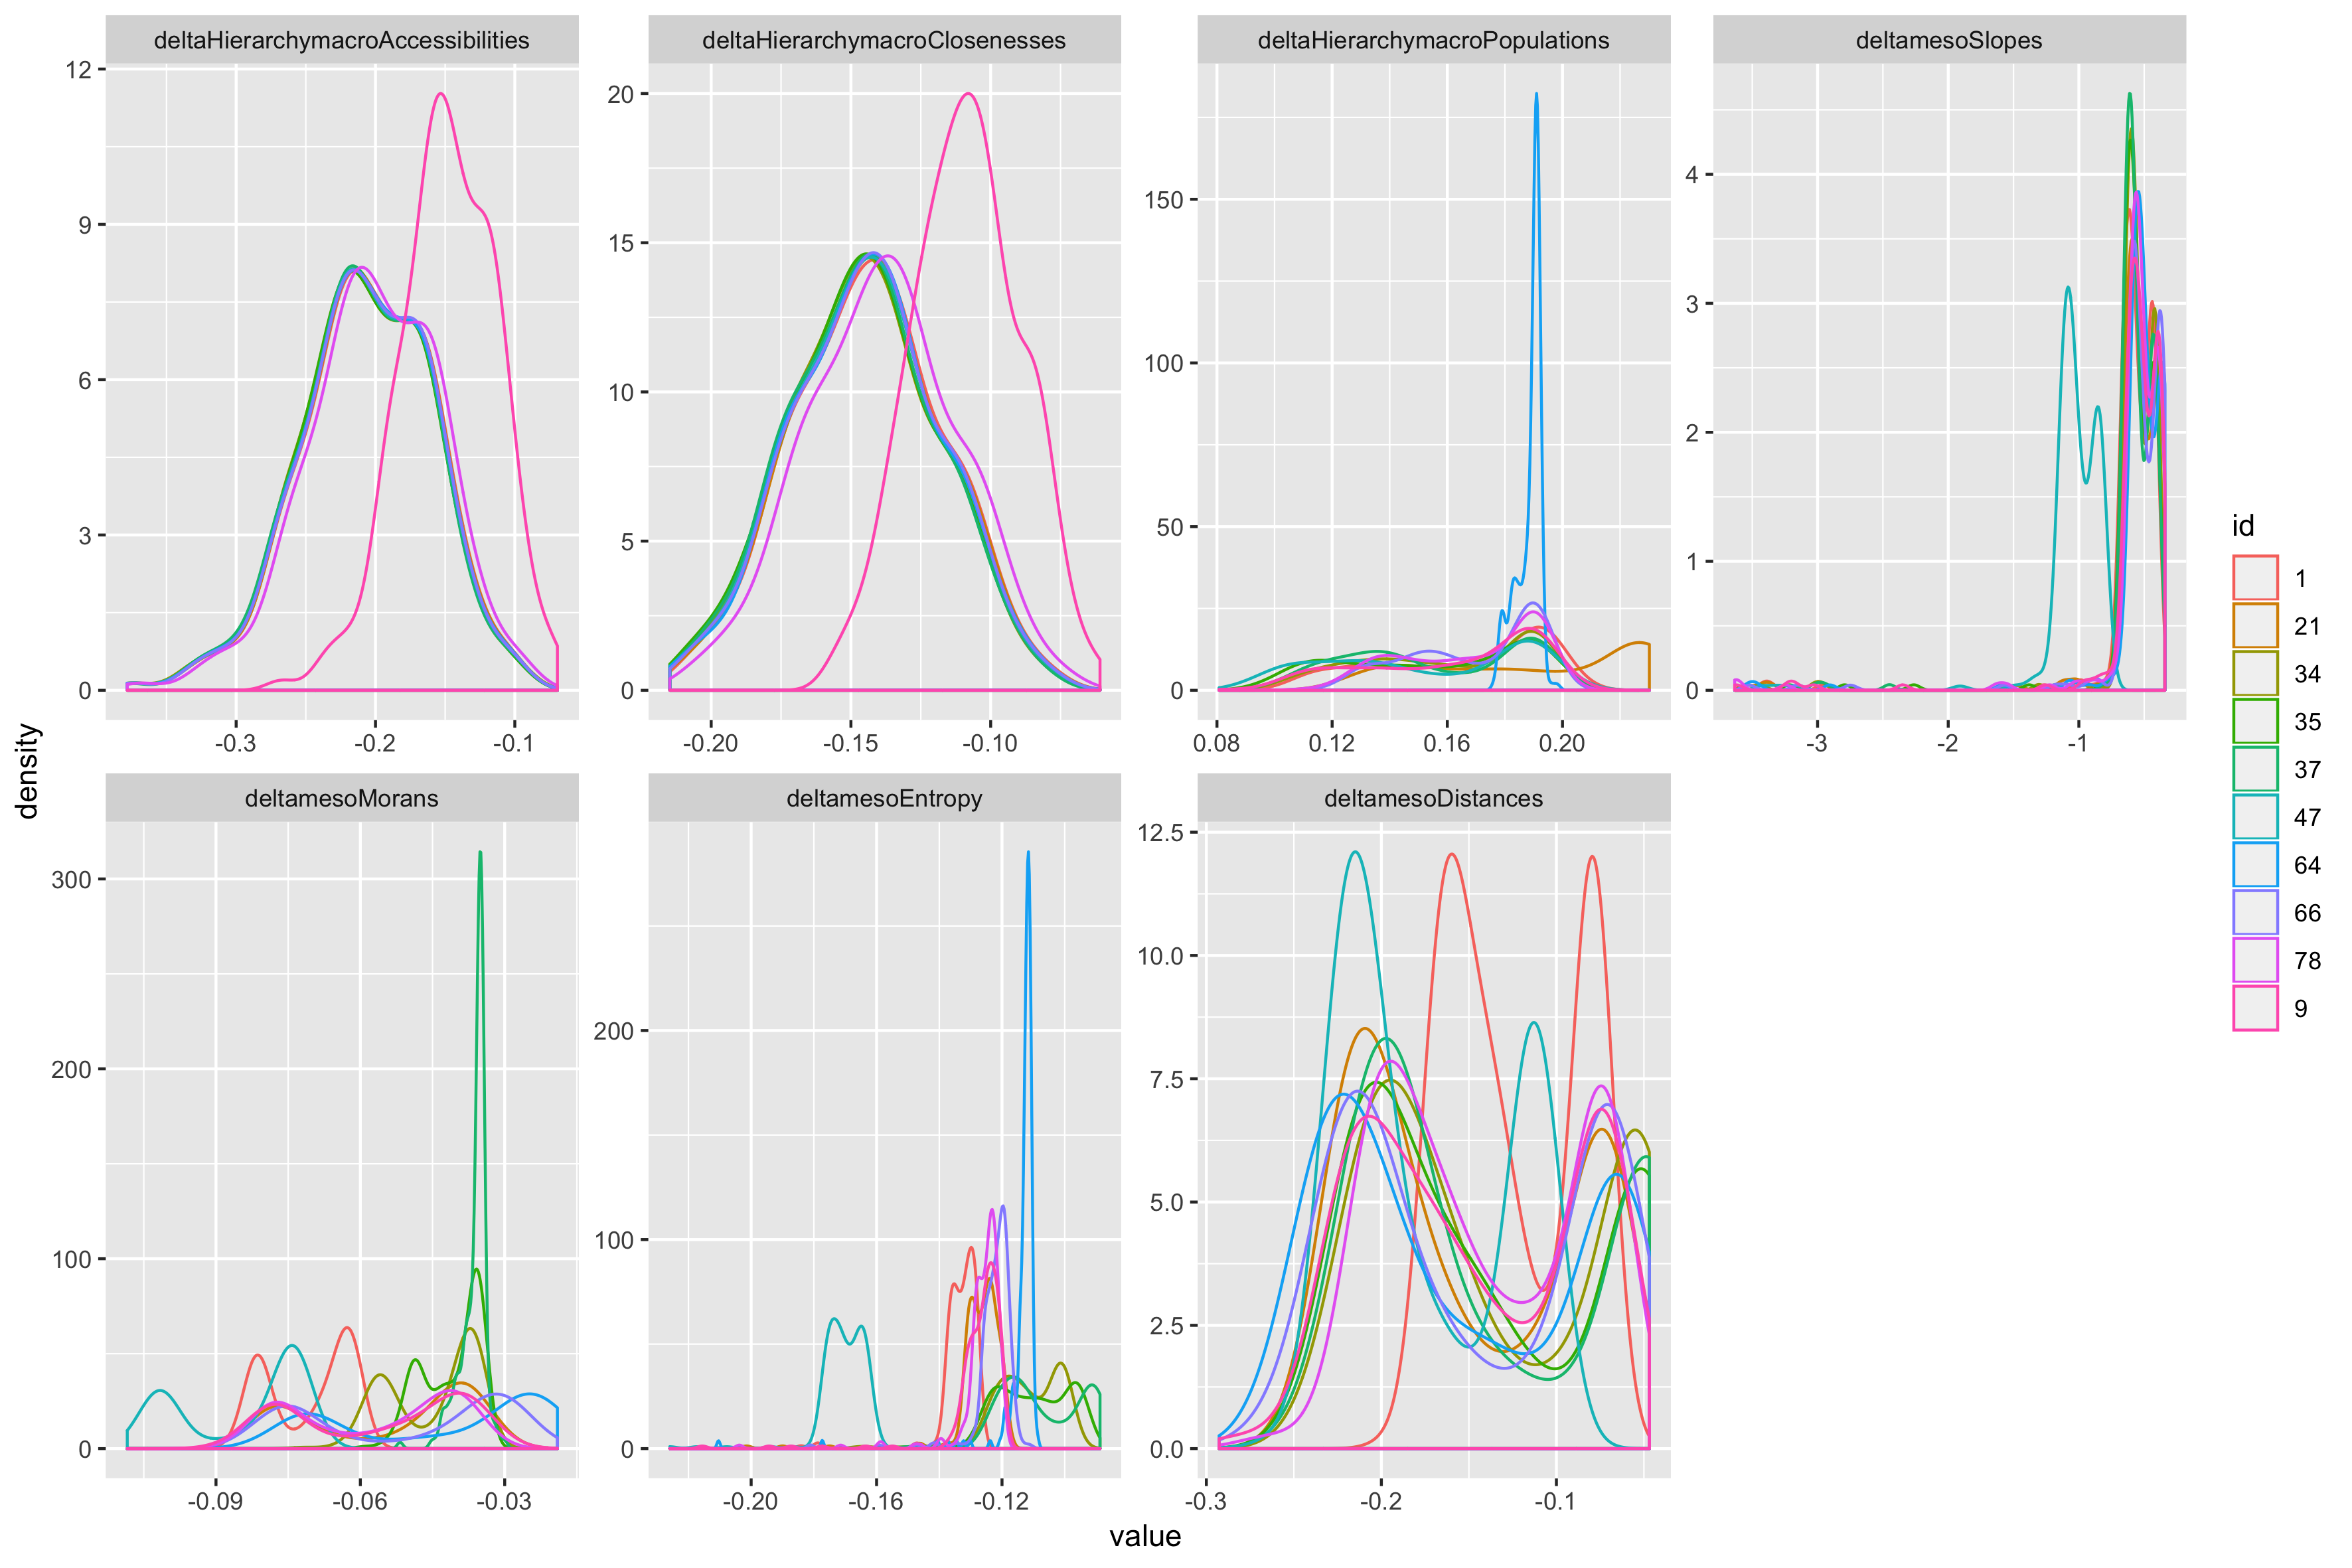
\includegraphics[width=0.8\textwidth]{figures/allindics_hist.png}
\end{center}

\textit{For all indicators, median sharpe ratios computing for a parameter point across repetitions are all larger than 1.6}

\subsection{Grid exploration}


% 20190429_193158_MULTISCALE_GRID_GRID.csv

First results show a strong impact of the strong meso-macro coupling, such as for example a qualitative inversion of the behavior as a function of interaction range of macroscopic indicators trajectories when switching from a ``transit-oriented development'' scenario (negative feedback of population growth on diffusion) to a ``sprawl'' scenario (positive feedback). Similarly, mesoscopic urban form indicators are significantly influenced by the coupling process.

\begin{figure}
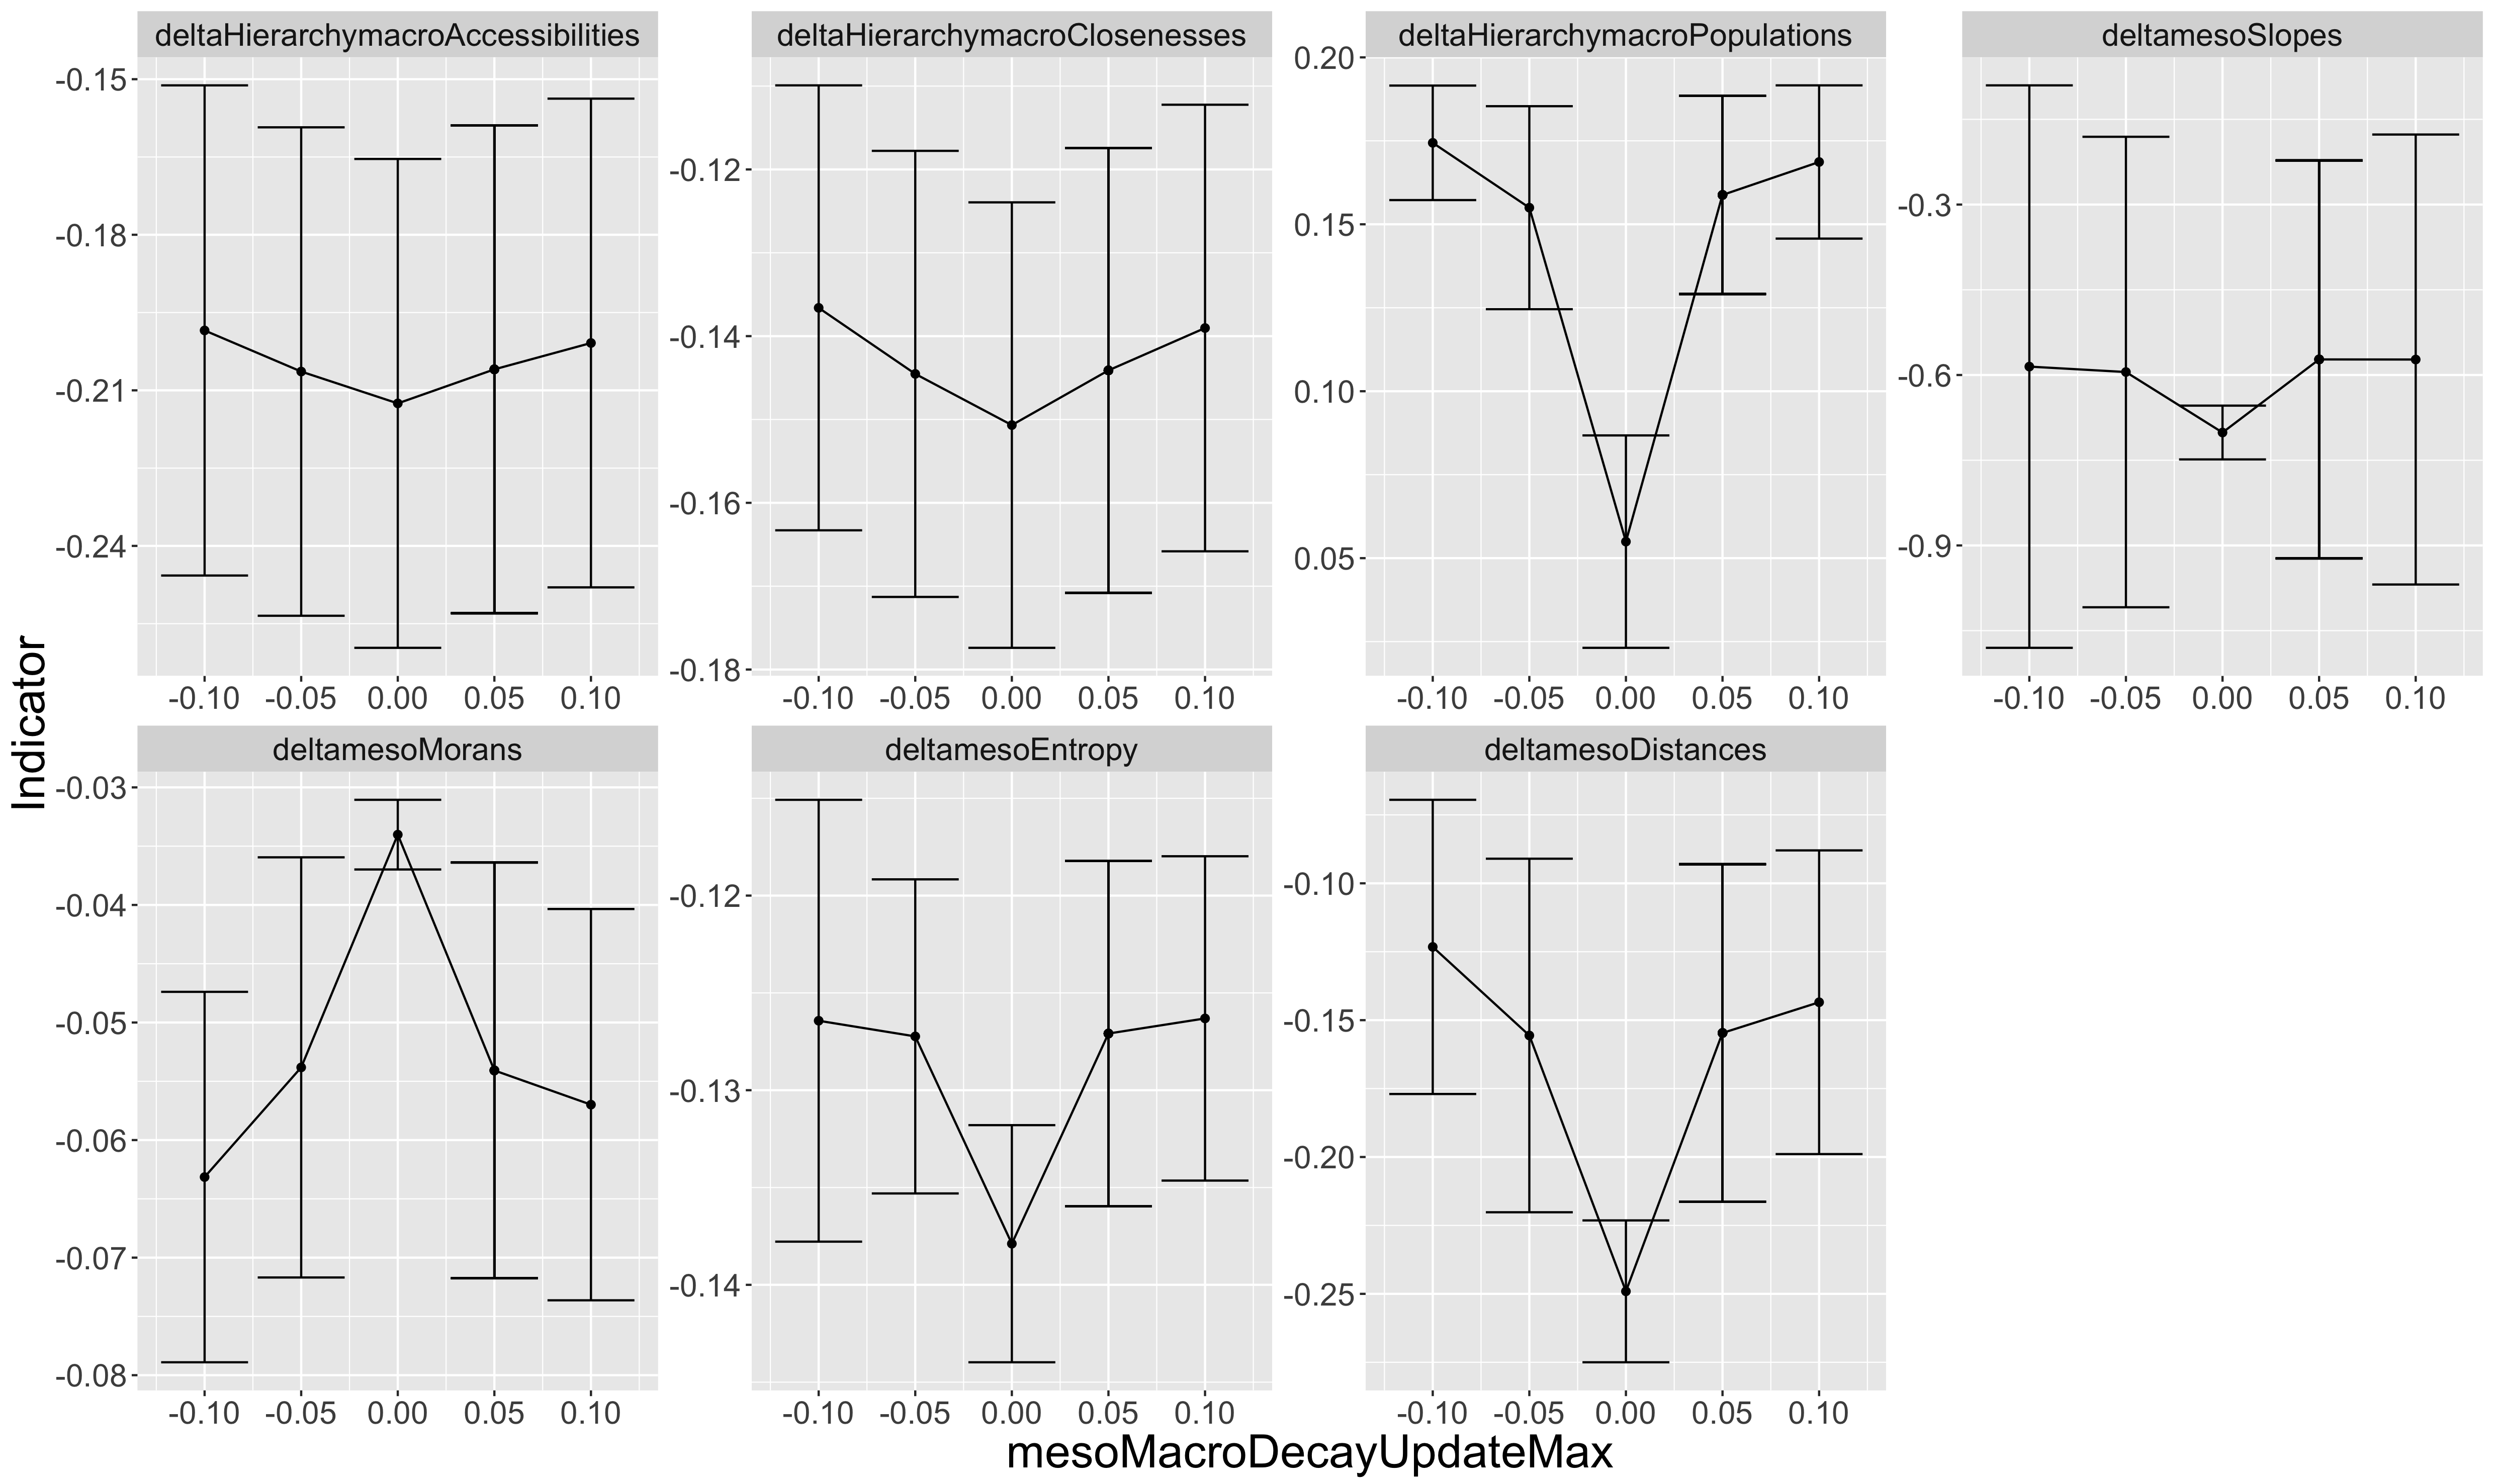
\includegraphics[width=\textwidth]{figures/onefactor_allindics_mesoMacroDecayUpdateMax_errorbars.png}
\end{figure}

\textit{U-shape behavior of both macroscopic and mesoscopic indicators as a function of $\delta d$}


% 20190506_135221_MULTISCALE_TARGETEDGRID_GRID

We do a targeted experiment to look at the influence of the macroscopic interaction decay and the mesoscopic evolution speed, under stylized scenarios for the downward feedback.

We run 50 replications for each parameter value.

Congestion cost for upward feedback is fixed to a rather strong effect.
% note : we should control here compare with / without feedback ?
%  -> first thing to check : with/ without the model

\begin{figure}
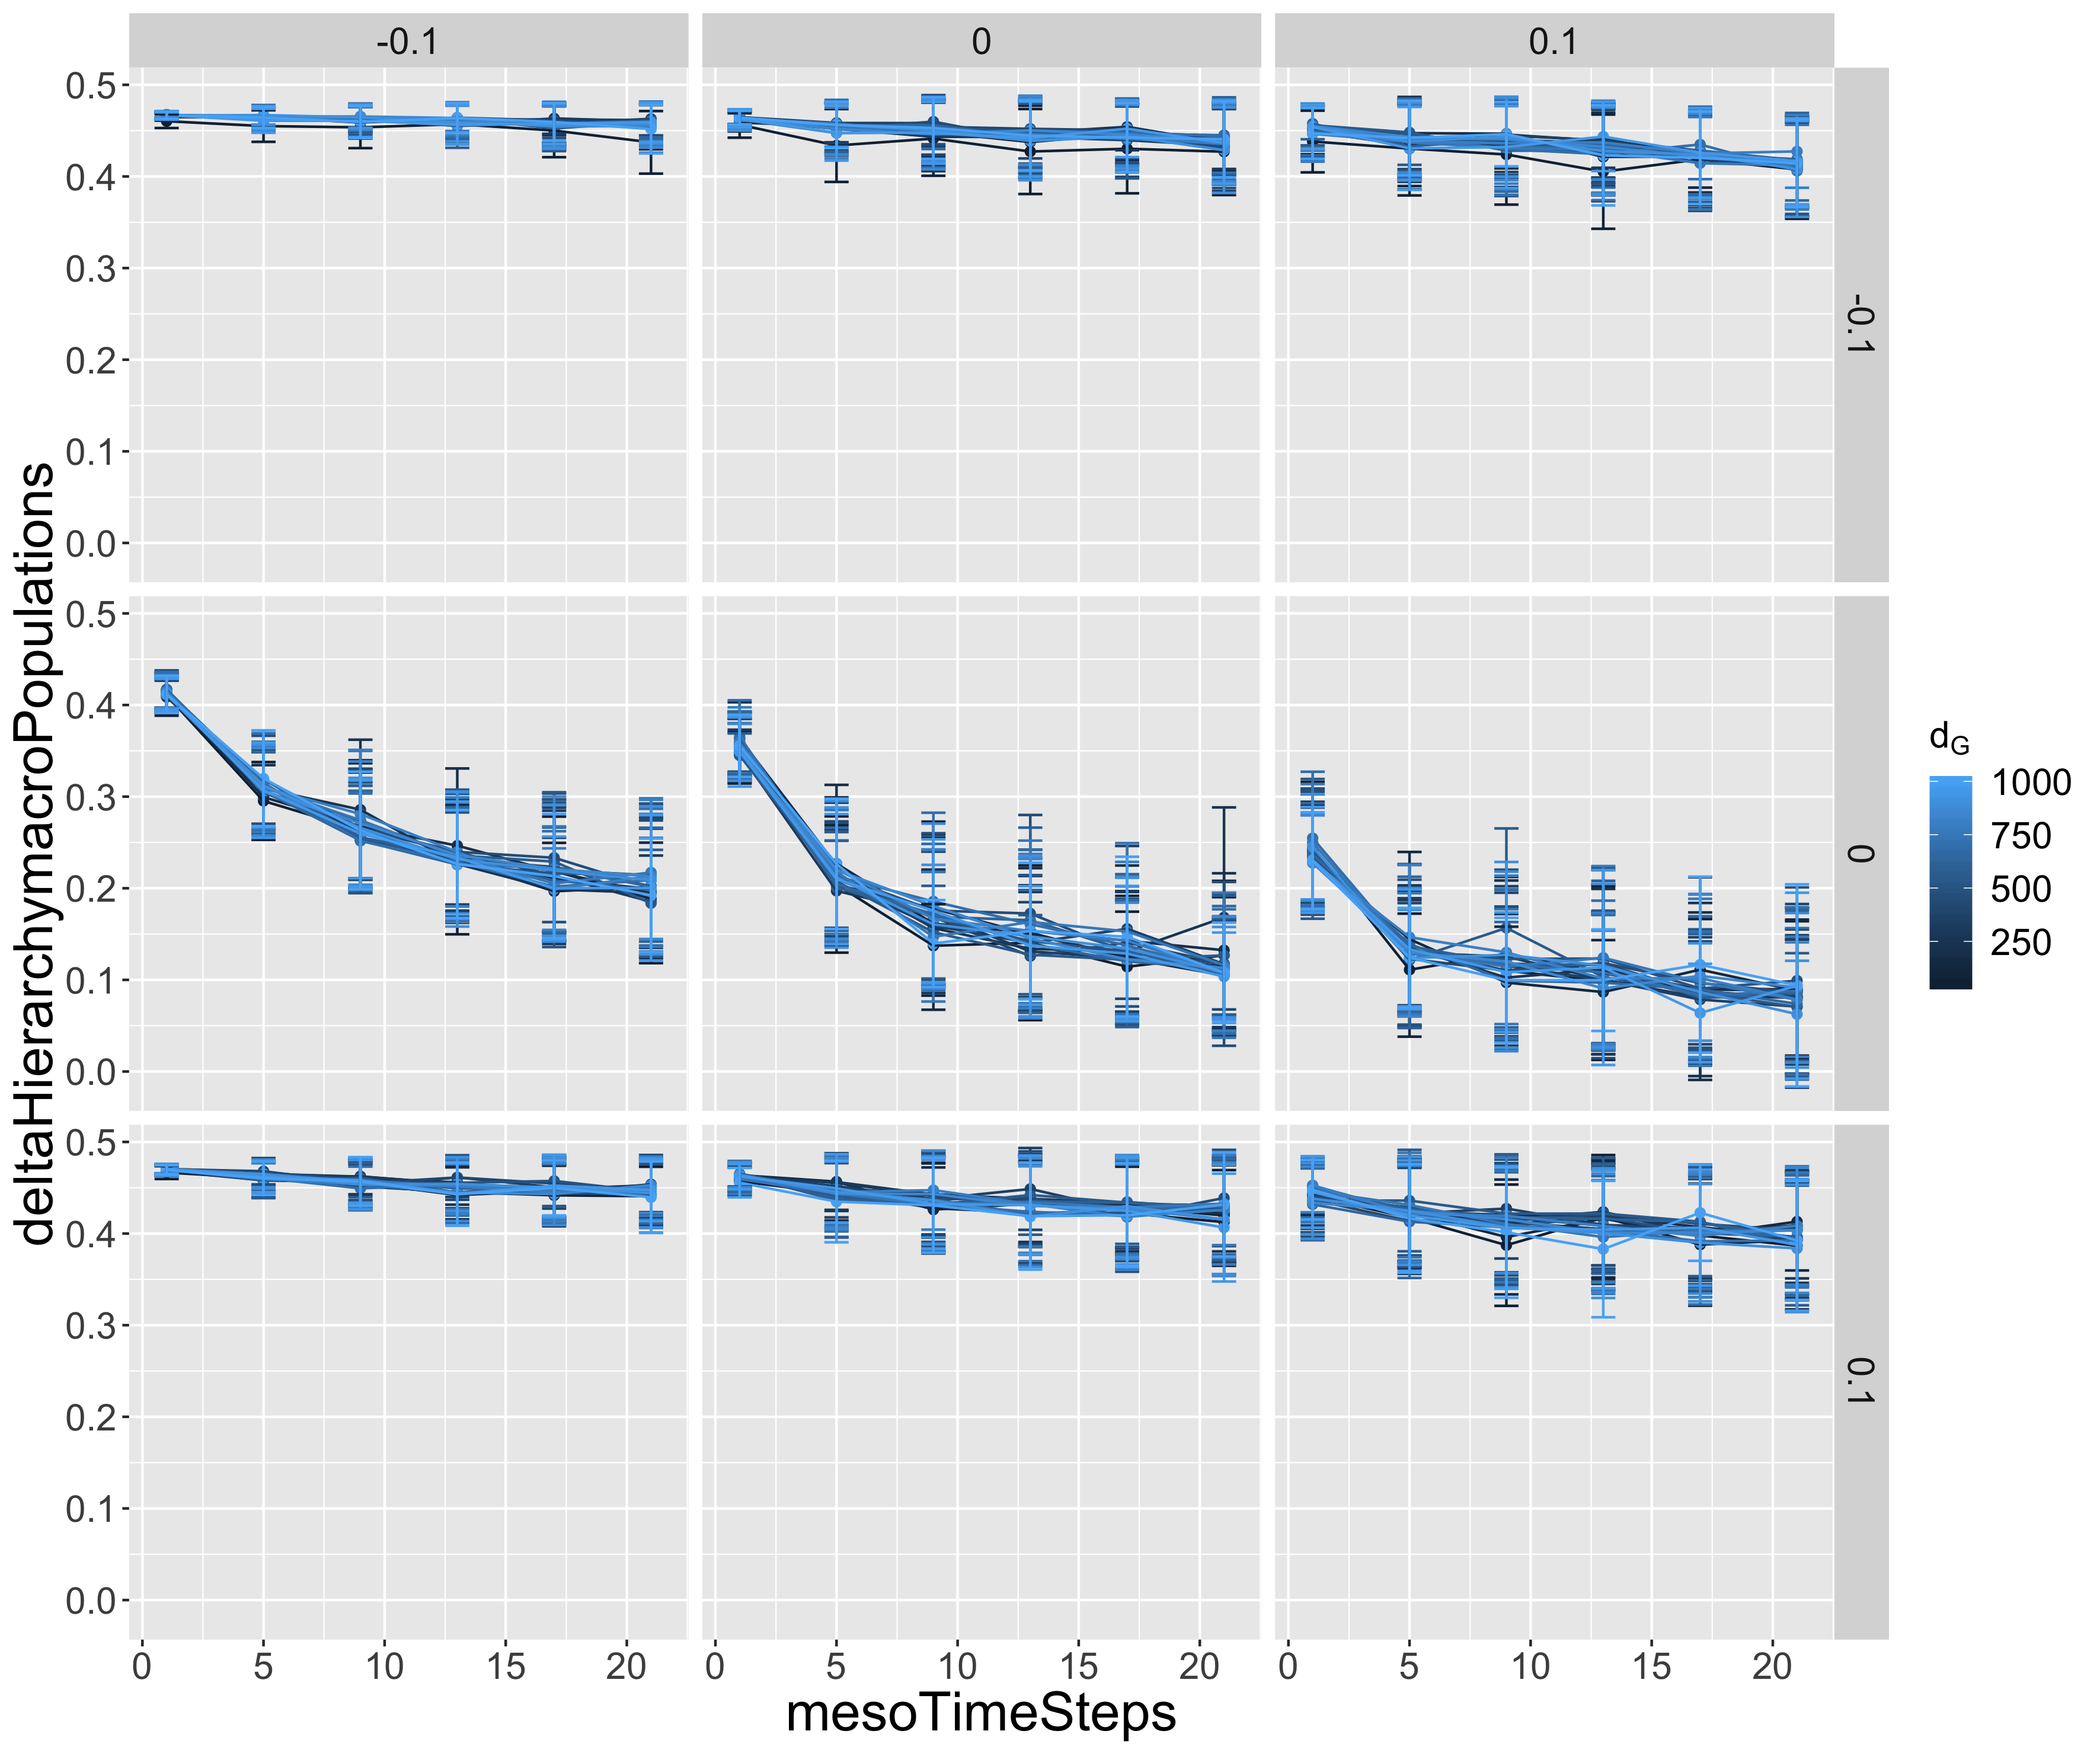
\includegraphics[height=0.75\textheight]{figures/deltaHierarchymacroPopulations-mesoTimeSteps_colorMacroInteractionDecay_facetmesoMacroDecayUpdateMax-macroMesoBetaUpdateMax.png}
\end{figure}

\textit{Non-trivial influence of coupled feedbacks on the different scales}



\subsection{Impact of policy parameters}


\begin{figure}
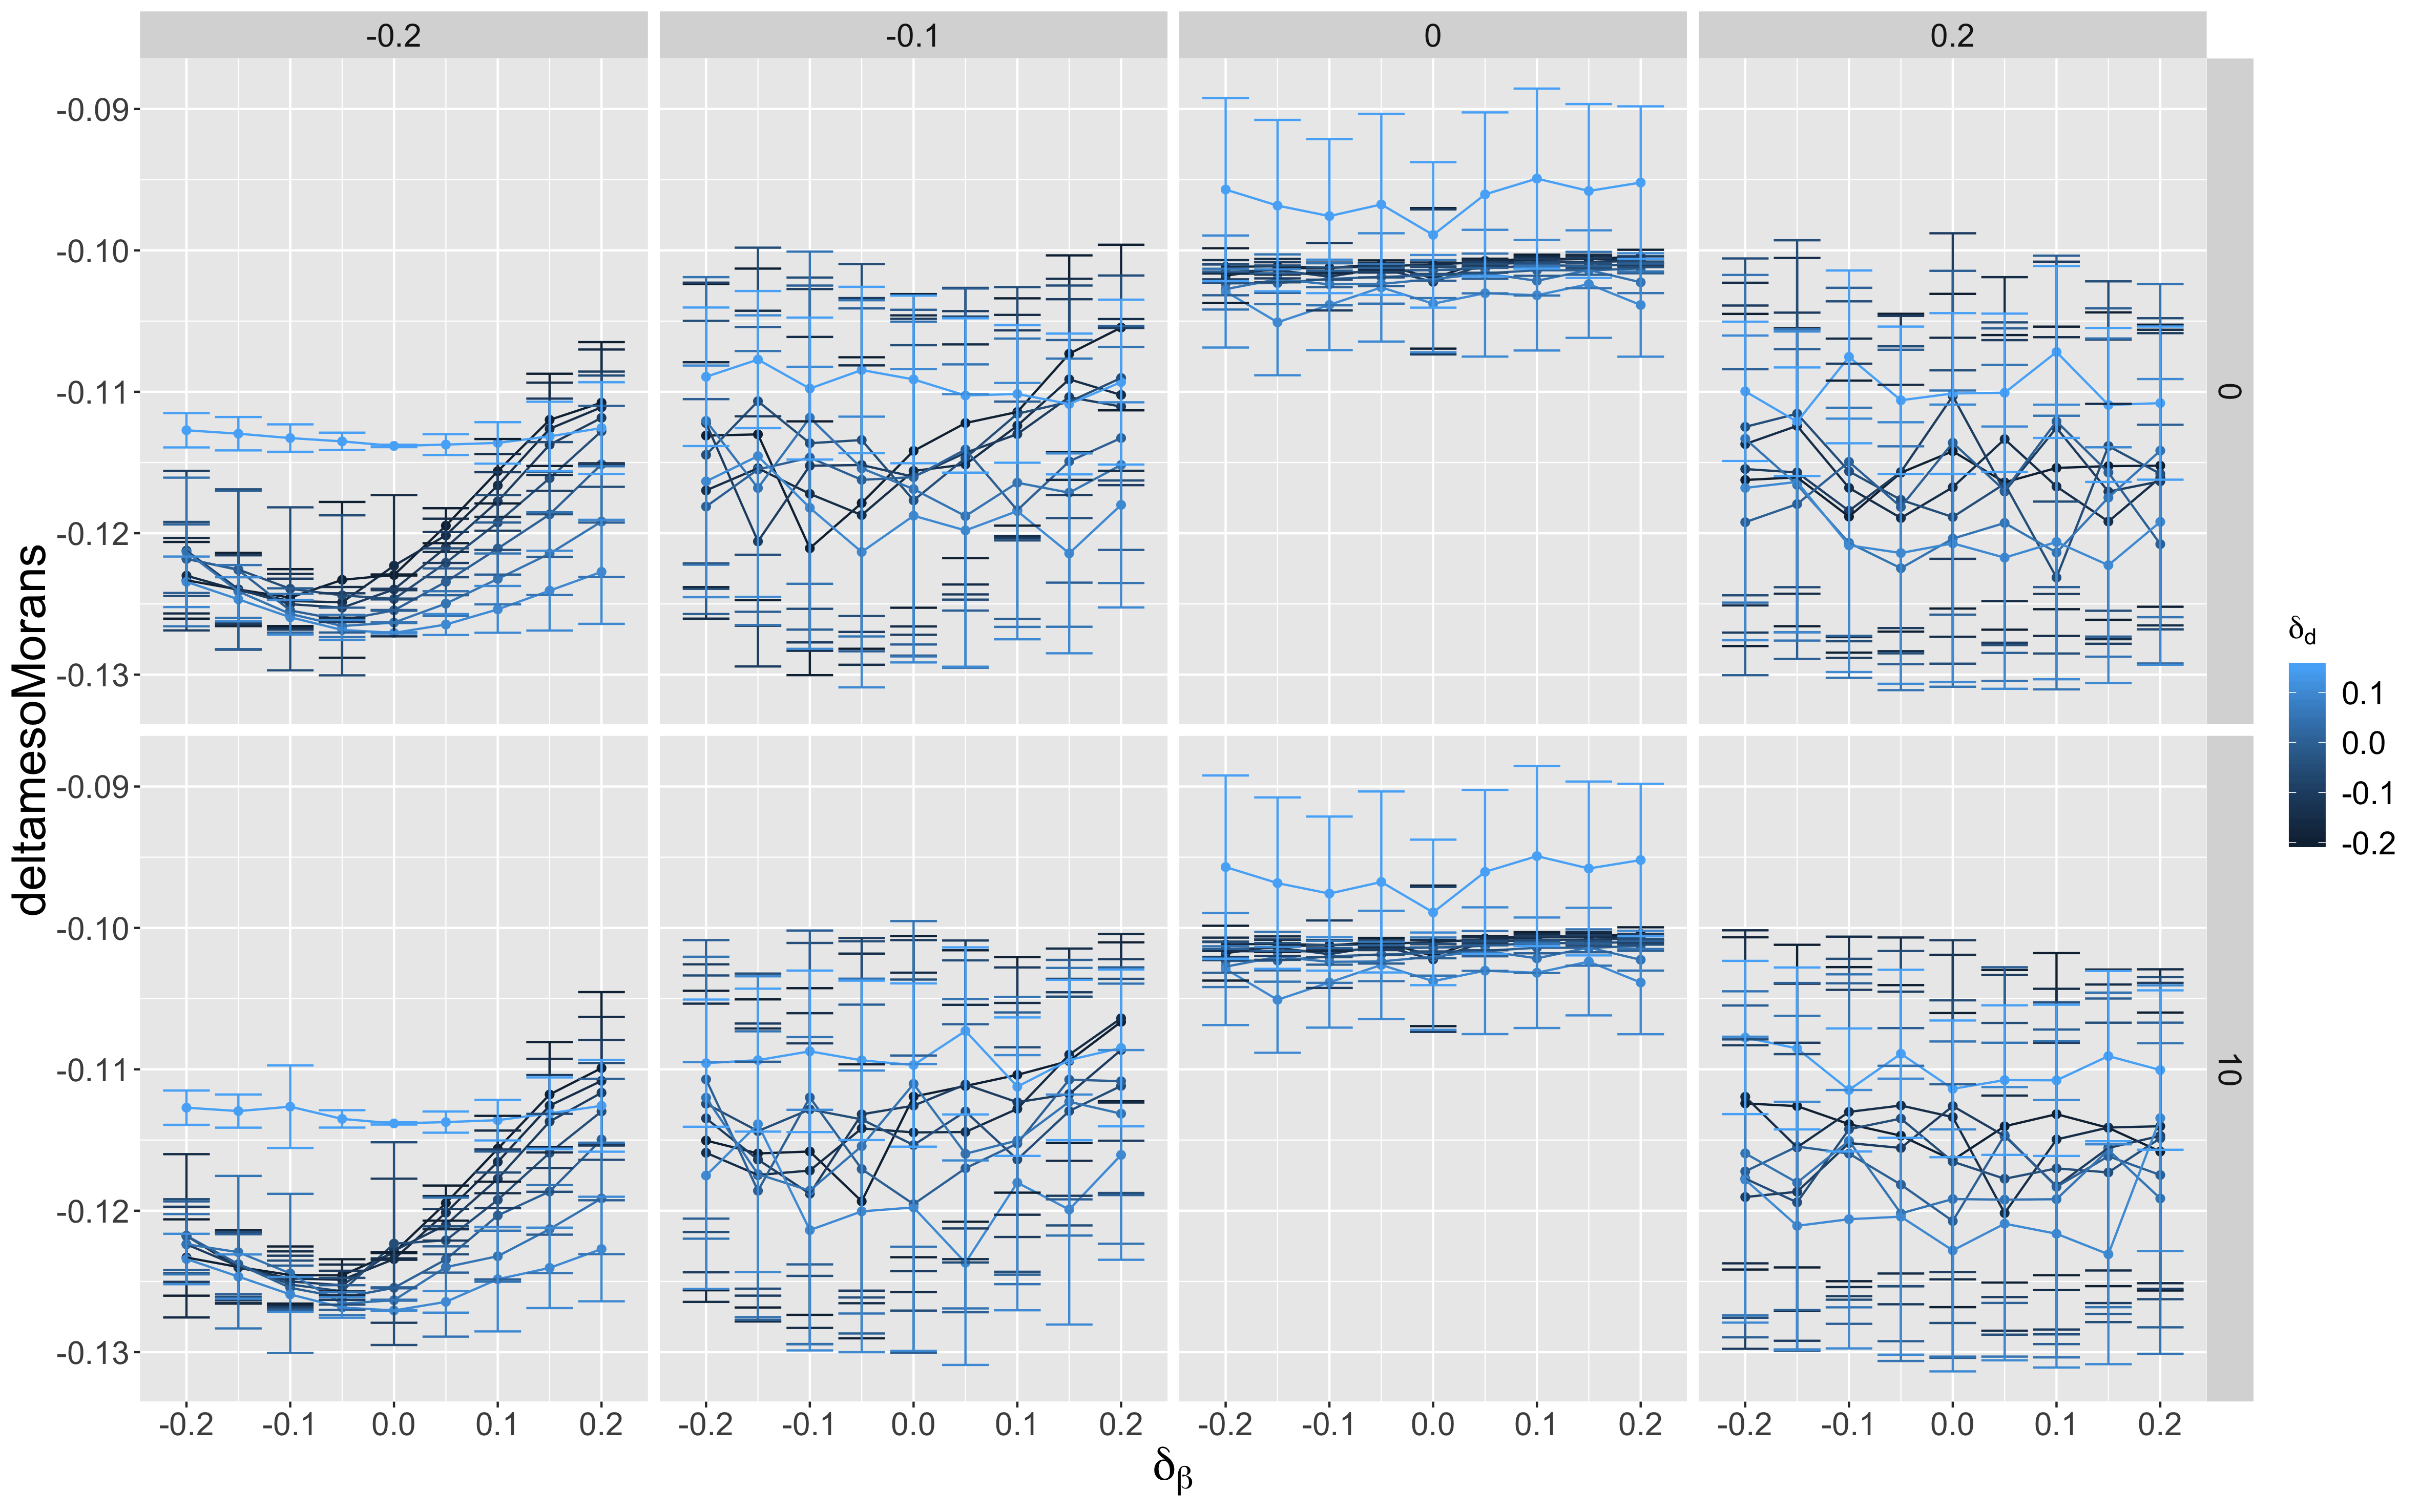
\includegraphics[height=0.7\textheight]{figures/deltamesoMorans-macroMesoAlphaUpdateMax_colormacroMesoBetaUpdateMax_facetmesoMacroCongestionCost-mesoMacroDecayUpdateMax_mesoBeta0_11.png}
\end{figure}

\textit{Mesoscopic centralization appears at a $\delta \beta$ critical value for low $\delta \alpha$; influenced by upward feedback}


\begin{figure}
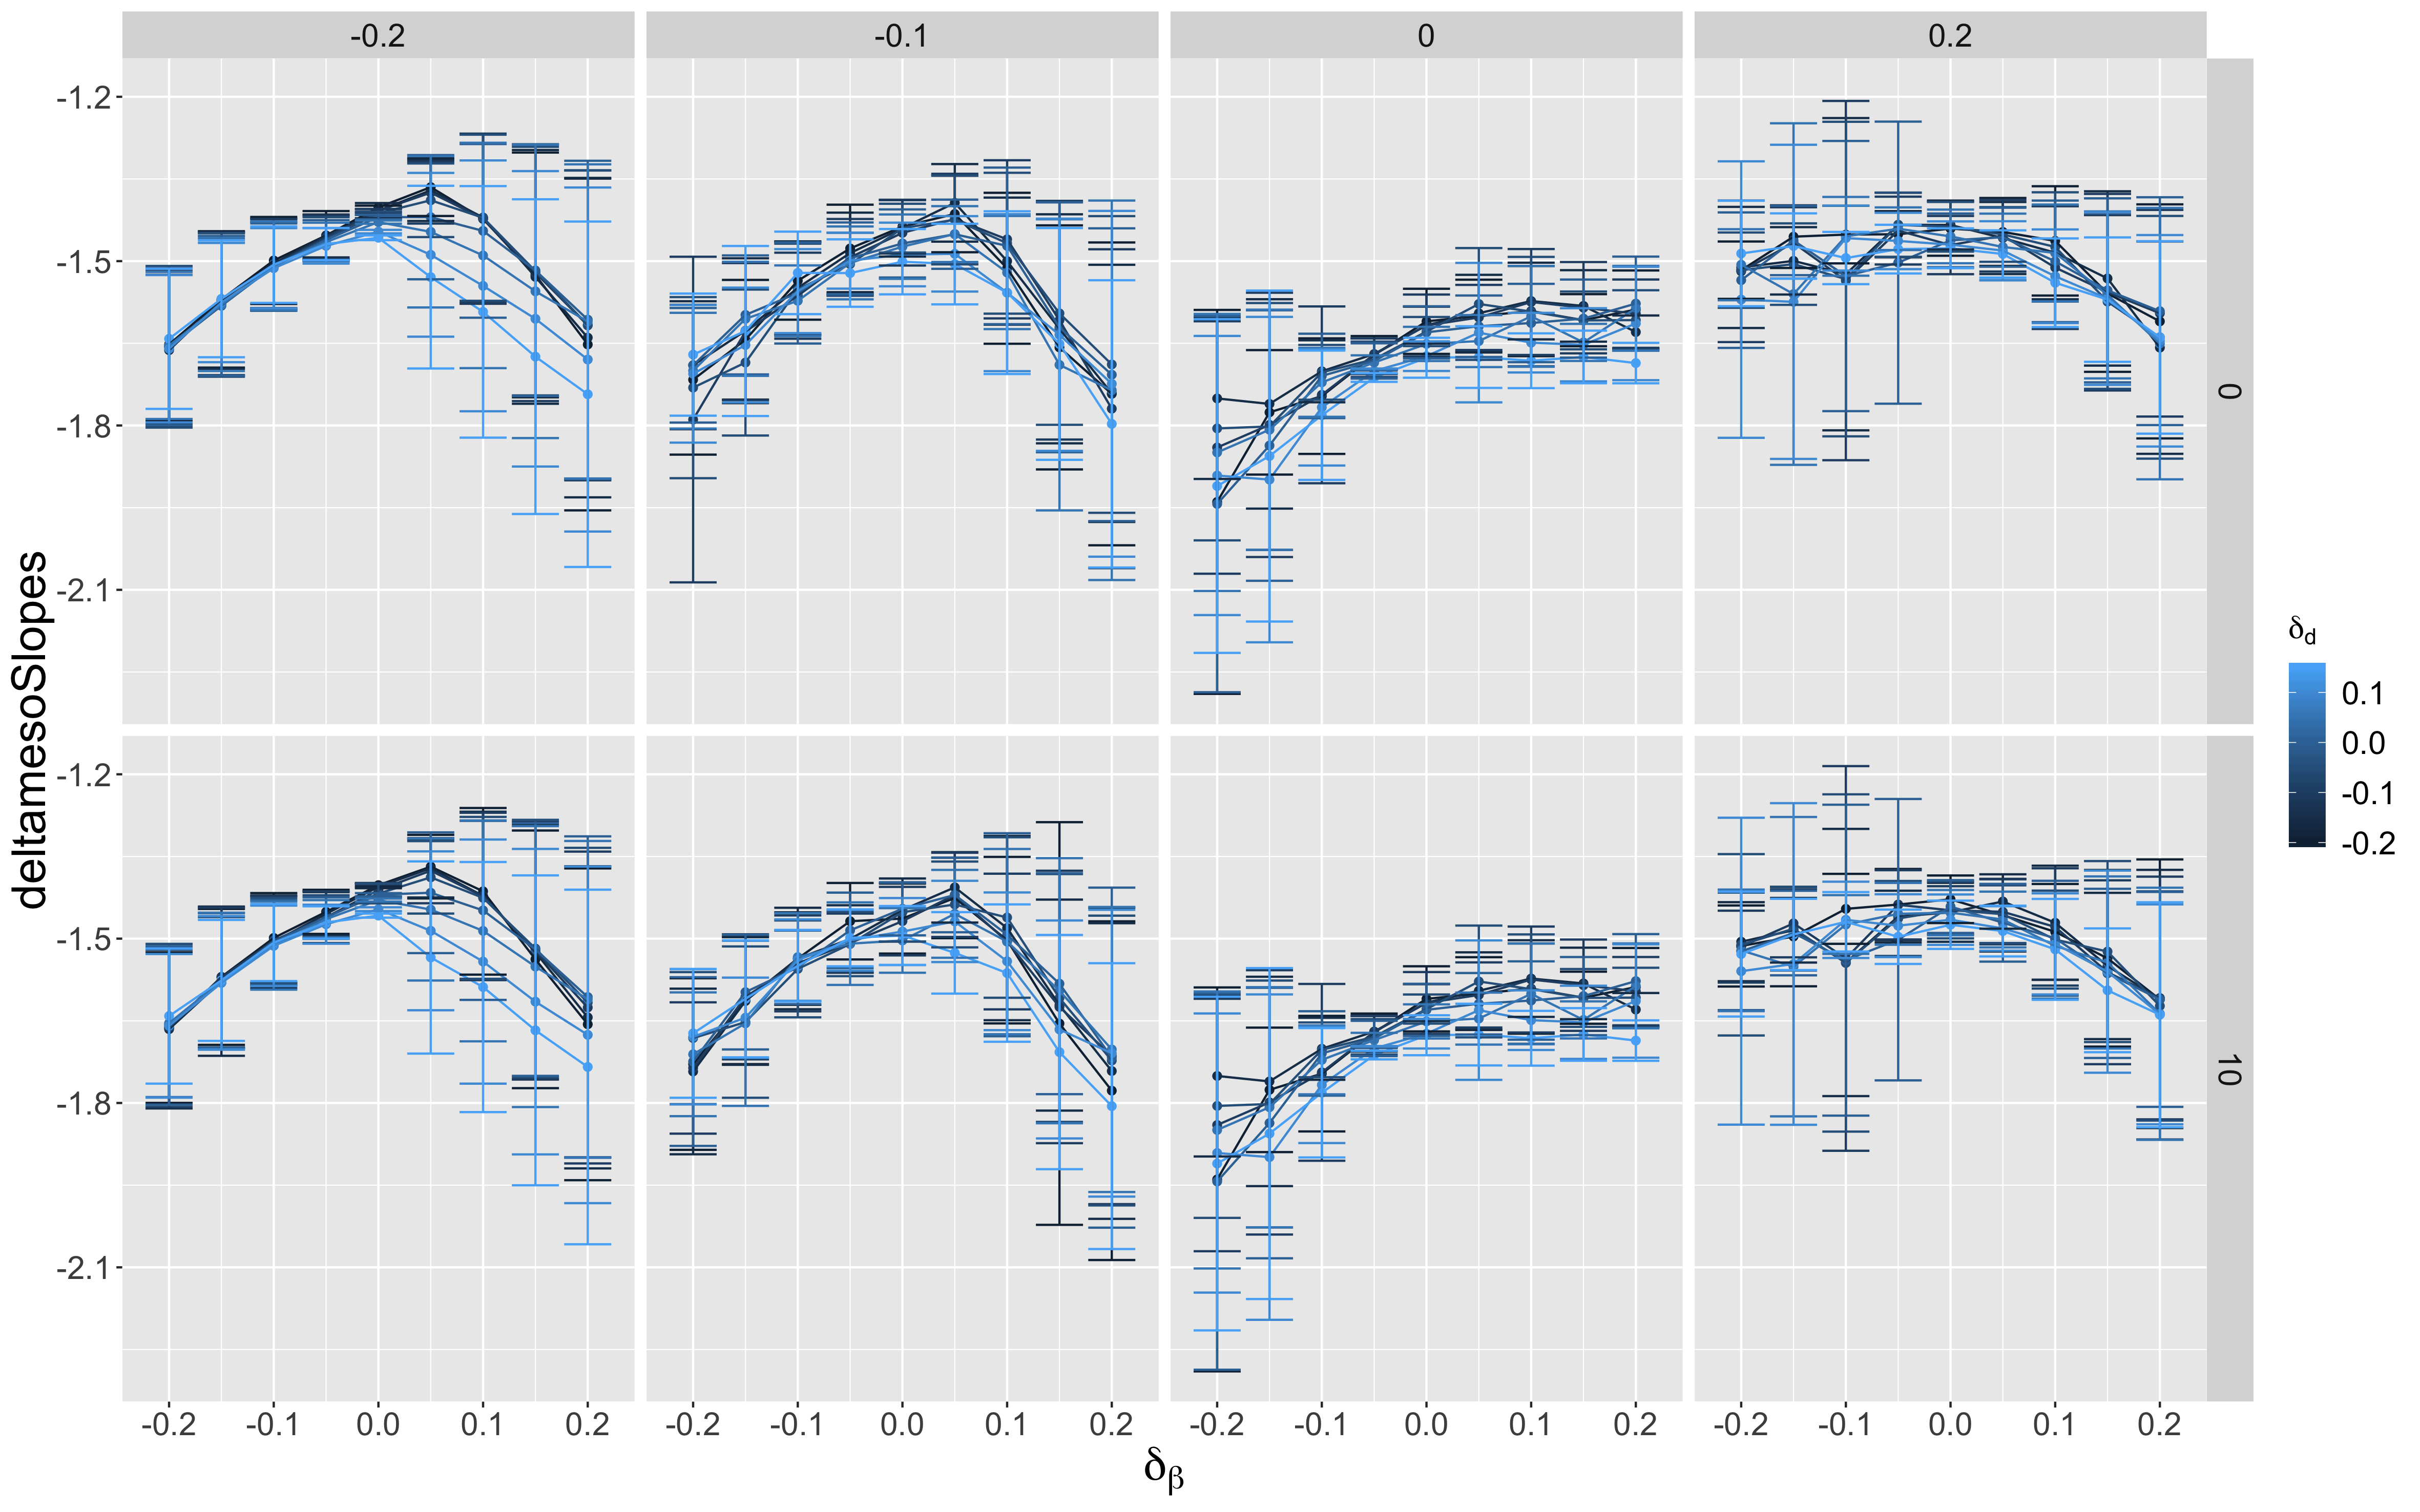
\includegraphics[height=0.7\textheight]{figures/deltamesoSlopes-macroMesoAlphaUpdateMax_colormacroMesoBetaUpdateMax_facetmesoMacroCongestionCost-mesoMacroDecayUpdateMax_mesoBeta0_11.png}
\end{figure}

\textit{Mesoscopic hierarchy has a U-shape of $\delta \beta$ in negative $\delta \alpha$, but has a plateau for positive values} 
%$\rightarrow$ sprawl is needed in a sense


\subsection{Multiscale optimization}

\begin{figure}
	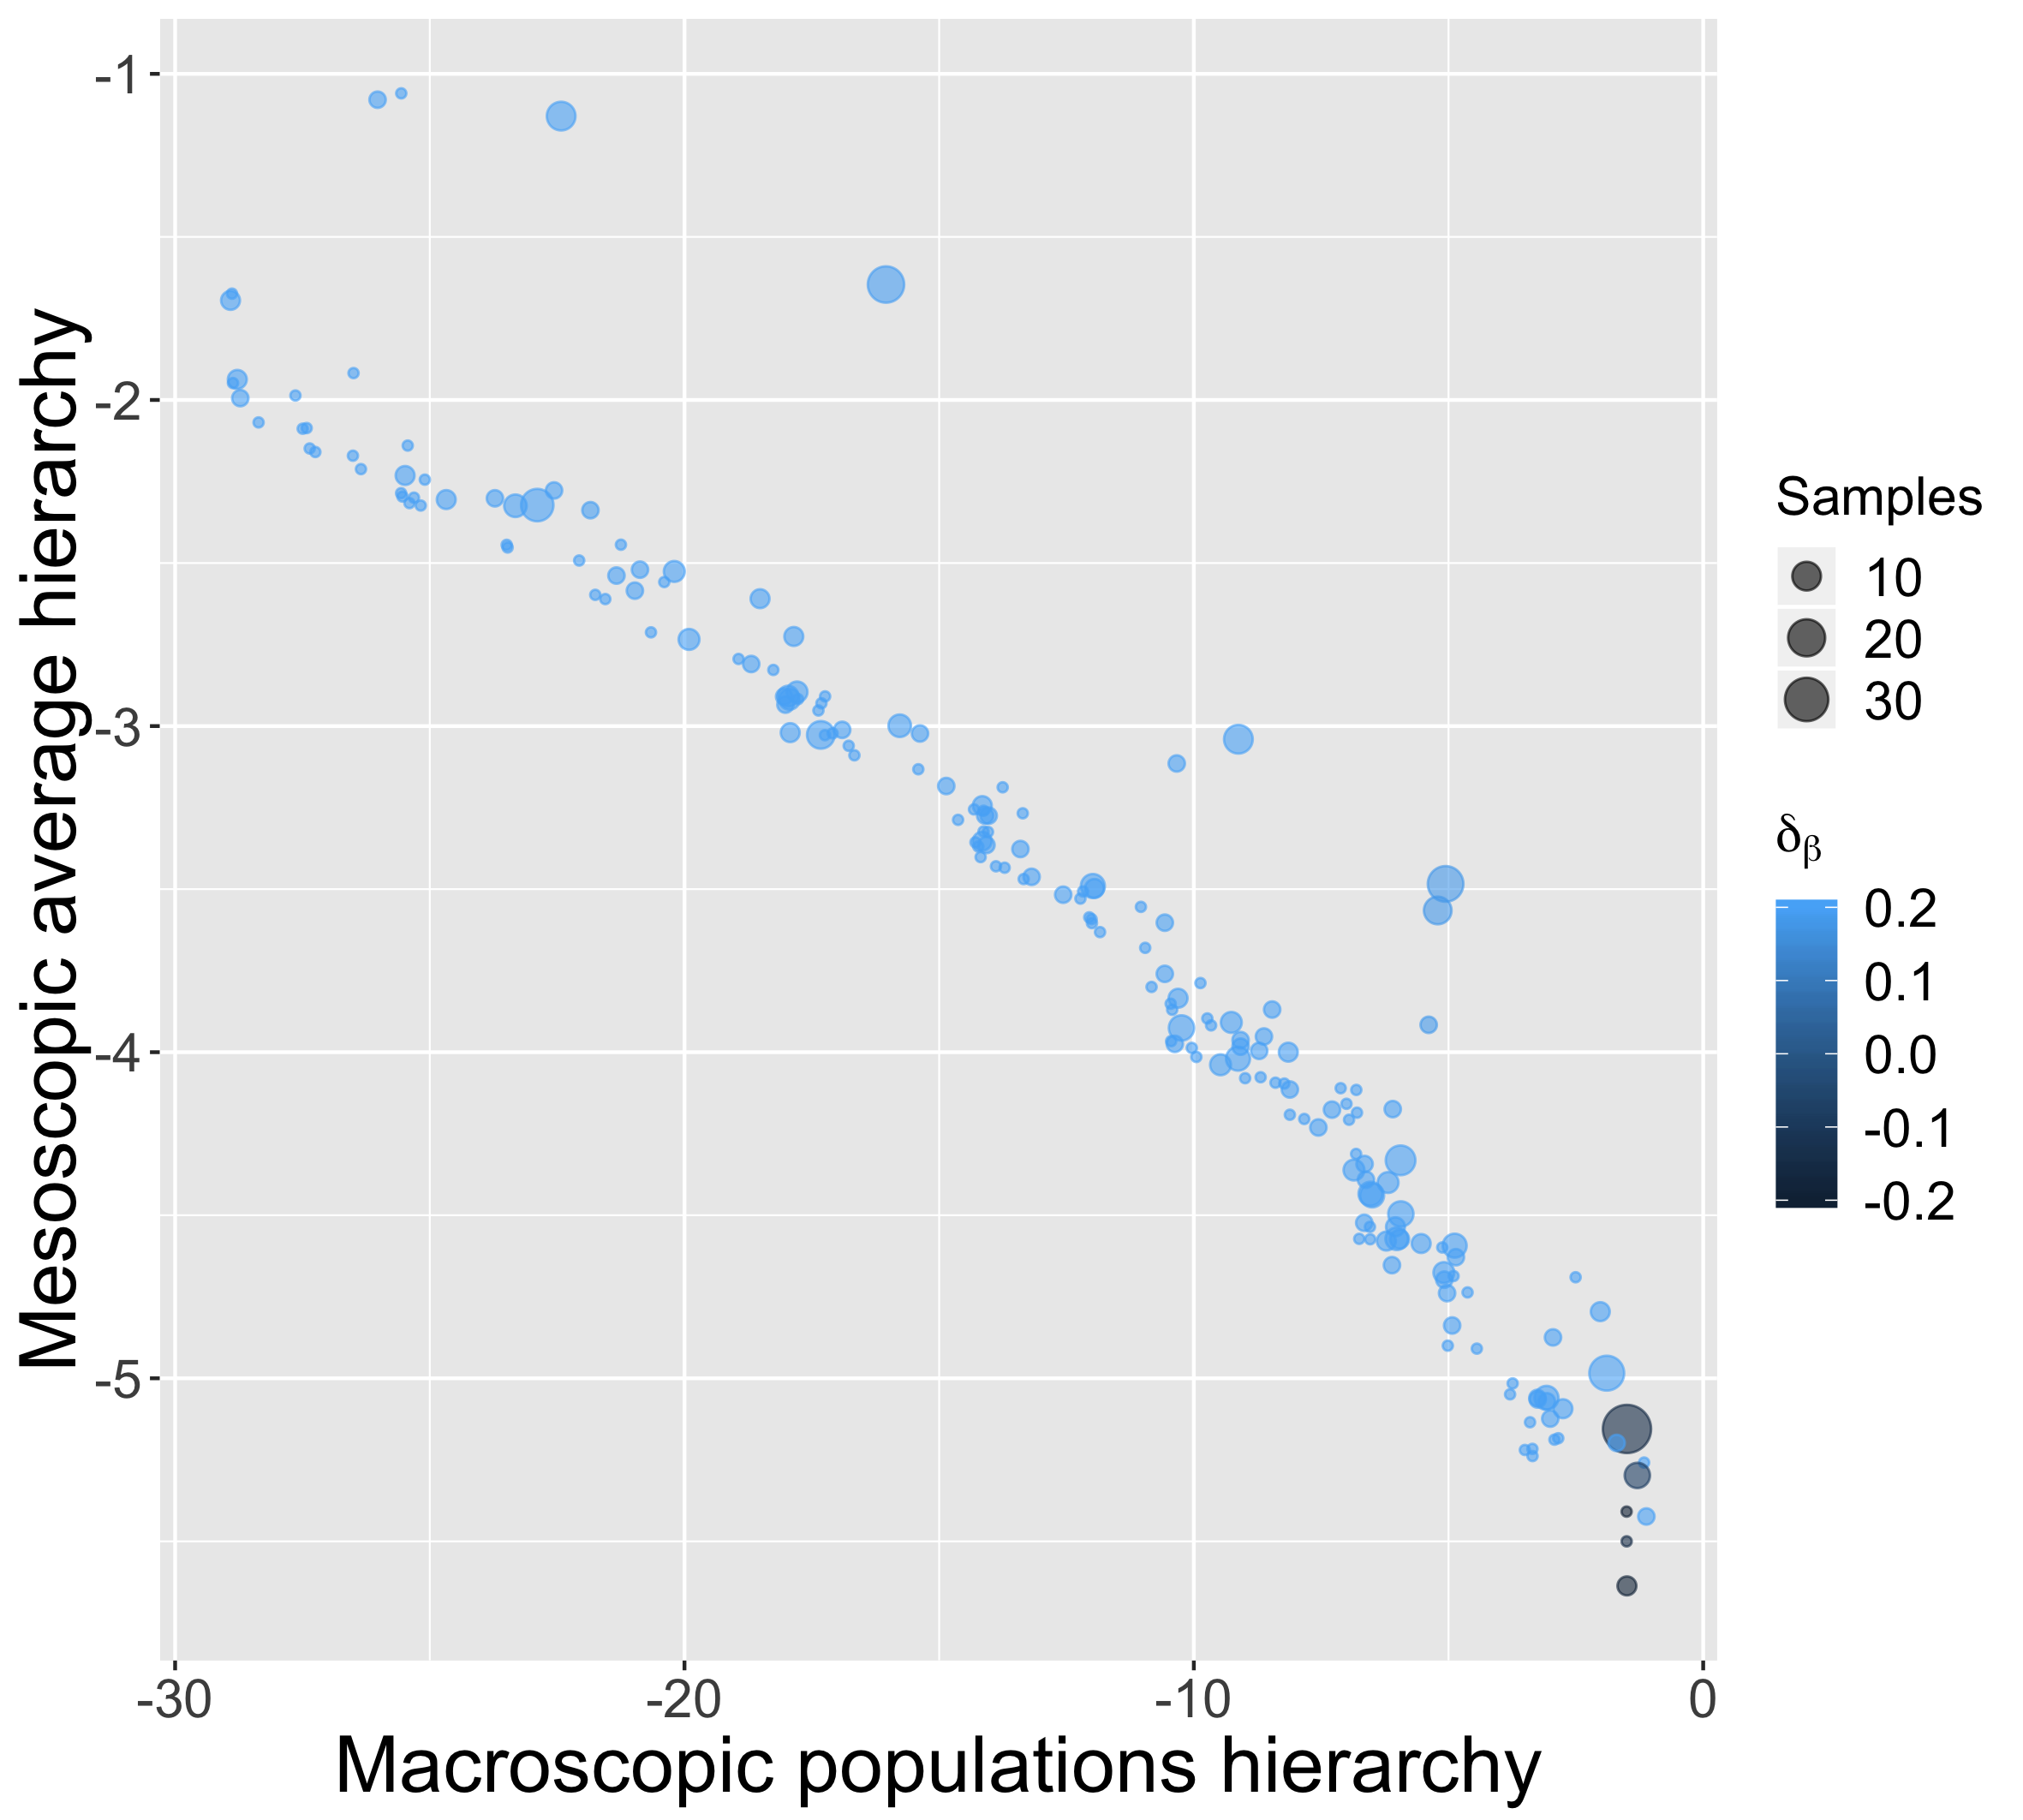
\includegraphics[width=0.8\textheight]{figures/pareto_macroHierarchy-mesoHierarchy.png}
\end{figure}

\textit{Pareto front obtained with Genetic Algorithm optimization for two contradictory objective of macrosopic and mesoscopic hierarchies}



\section{Discussion}


\subsection{Multi-modeling and concurrent processes}

This model is only a first structural sketch with very restrictive assumption, in particular regarding the downward and upward feedbacks on submodel parameters. There may be no link between urban form and global insertion, or it may be due to other processes, be expressed as an other functional form. An important stage before shifting to robust knowledge will consist in (i) reviewing and making a typology of such potential processes across scales; (ii) including most in a multi-modeling fashion to compare possible concurrent mechanisms.


\subsection{Developments}

Further work will consist in more targeted simulation experiments, including specific exploration algorithms such as diversity search for model regimes \cite{reuillon2013openmole}, to test the model as a proof-of-concept of models for policies. Such a model can also be calibrated on real city systems and urban form trajectories, to extrapolate coupling parameters that would be difficult to obtain otherwise. Our contribution is thus a first step towards multi-scalar simulation models for systems of cities.

We also did not include explicitly transportation networks in this model.


\textbf{Theoretical and practical implications}



$\rightarrow$ model effectively captures an interaction between downward and upward feedback: weak emergence \cite{bedau2002downward}



$\rightarrow$ coupling ``simple three parameters models'' yield a complicated and complex simulation model: necessity of complexity and simulation models to understand urban complexity? 
% 'suggest in a way failure of reductionist empistemology (in the sense of a la Barthelemy) - at least for grabbing the multi-scalar nature of systems' (seems a tautology though


$\rightarrow$ progressive integration towards models for policy?


\textbf{Developments}

$\rightarrow$ diversity search algorithm to find e.g. regimes with the strongest effect of feedback


$\rightarrow$ parametrization on real systems; possibly calibration

\cite{raimbault2019ilus}




\section{Conclusion}

A first step towards \textit{strongly} multi-scalar models to capture urban complexity towards policy models

 Towards integrative models and theories for urban systems \cite{raimbault2019methods}

\textbf{Acknowledgments}: thanks to the \textit{European Grid Infrastructure} for access to the infrastructure.




\bibliographystyle{apalike}
\bibliography{biblio}


\end{document} 
